\subsubsection{Latency \& Throughput}

Charts on Figures \ref{fig:sequential_transport_latency}, \ref{fig:parallel_transport_latency}, \ref{fig:sequential_transport_throughput} and \ref{fig:parallel_transport_throughput} represent the \gls{p90} of Latency and Throughput of all 10000 requests made by the parallel and sequential clients during the experiments.

\subsubsection*{High Parallel Client Latency}

As seen in the chart on Figures \ref{fig:sequential_transport_latency} and \ref{fig:parallel_transport_latency}, both parallel and sequential clients possess a similar behavior. Their scale is differ, however. 

Parallel clients results show a hundredfold difference. They run 100 goroutines at the same time, increasing the time each request takes to complete since segments are send in sequence due to only having one connection with the server. Consequently, latency increases 100 times since each goroutine needs to wait for the other 99 to complete their requests before sending any actual data.

\subsubsection*{Multi-AZ Higher Throughput}

As performing Multi-AZ requests have increased latency when compared to others, sequential clients had their throughput affected during experiments. Nonetheless, parallel experiments were not affected by higher latency. Parallel requests do have a higher latency when compared individually, but latency is not the bottleneck.

As many requests are made at the same time, the throughput is defined by how fast requests leave the client and server's response time. Therefore, latency does not impact as much as it did during sequential experiments. Consequently, all three scenarios, Local, Same-AZ, and Multi-AZ, have a very similar result in their respective protocol.

\subsubsection*{Throughput Parallel Upper Limit}

During Parallel clients experiments TCP and TCP+TLS protocols throughput results were very similar. While sequential experiments throughputs showed these protocols can have a better performance, parallel requests seem to have a upper limit to how well they can perform.

Sequential experiments requests always have the client and server completely available to them, resulting in a immediate action when the client wants to send a request and when the server wants to send a response. Parallel experiments requests don't have that luxury, however. Multiple requests are made at the same time, requiring the client to queue requests coming out and responses coming in, the same happens to the server. Due to the amount of parallel requests, this queuing delay is enough to degrade throughput.

\subsubsection*{UDP Linux Restrictions}

QUIC's performance improved a bit overall when requests were made in parallel. Apart from the improvement in the Multi-AZ scenario, it remained roughly the same, however. This happens due to Linux restrictions to UDP performance \cite{linux_tuning}. 

The UDP receive buffer is responsible for holding packets that have been received by the kernel, but still were not read by the application \cite{udp_buffer_size_warning}. Once it fills up, the kernel will drop any new incoming packets. Usually, the UDP receive buffer size is 128KiB, enough for only 1 microsecond of data on a megabit network \cite{linux_tuning}.

Upon receiving a warning from QUIC's Go Implementation about the small buffer size, it was increased to 26MiB, more than the recommended amount, 2.5MB. Even though the buffer was increased significantly, QUIC still reached an upper throughput limit of 1Gb/s, explaining why both sequential and parallel experiments with 128KiB and 512KiB payloads resulted in almost the same value

\subsubsection*{UDP Failure}

During sequential experiments UDP succeeded during Local scenario throughout all packet sizes, failing in Same-AZ and Multi-AZ scenarios from 32 KiB payloads onward. Parallels experiments failed on all 32 KiB payloads onward, however. As 100 requests are performed at the same time, the UDP receive buffer from the server fills up faster than the application can read incoming messages, resulting in the kernel dropping any new incoming messages. Sequential experiments succeeded on Local scenario since they never overflow the UDP receive buffer, as only one request is performed at a time.

\clearpage

\begin{figure}
    \centering
    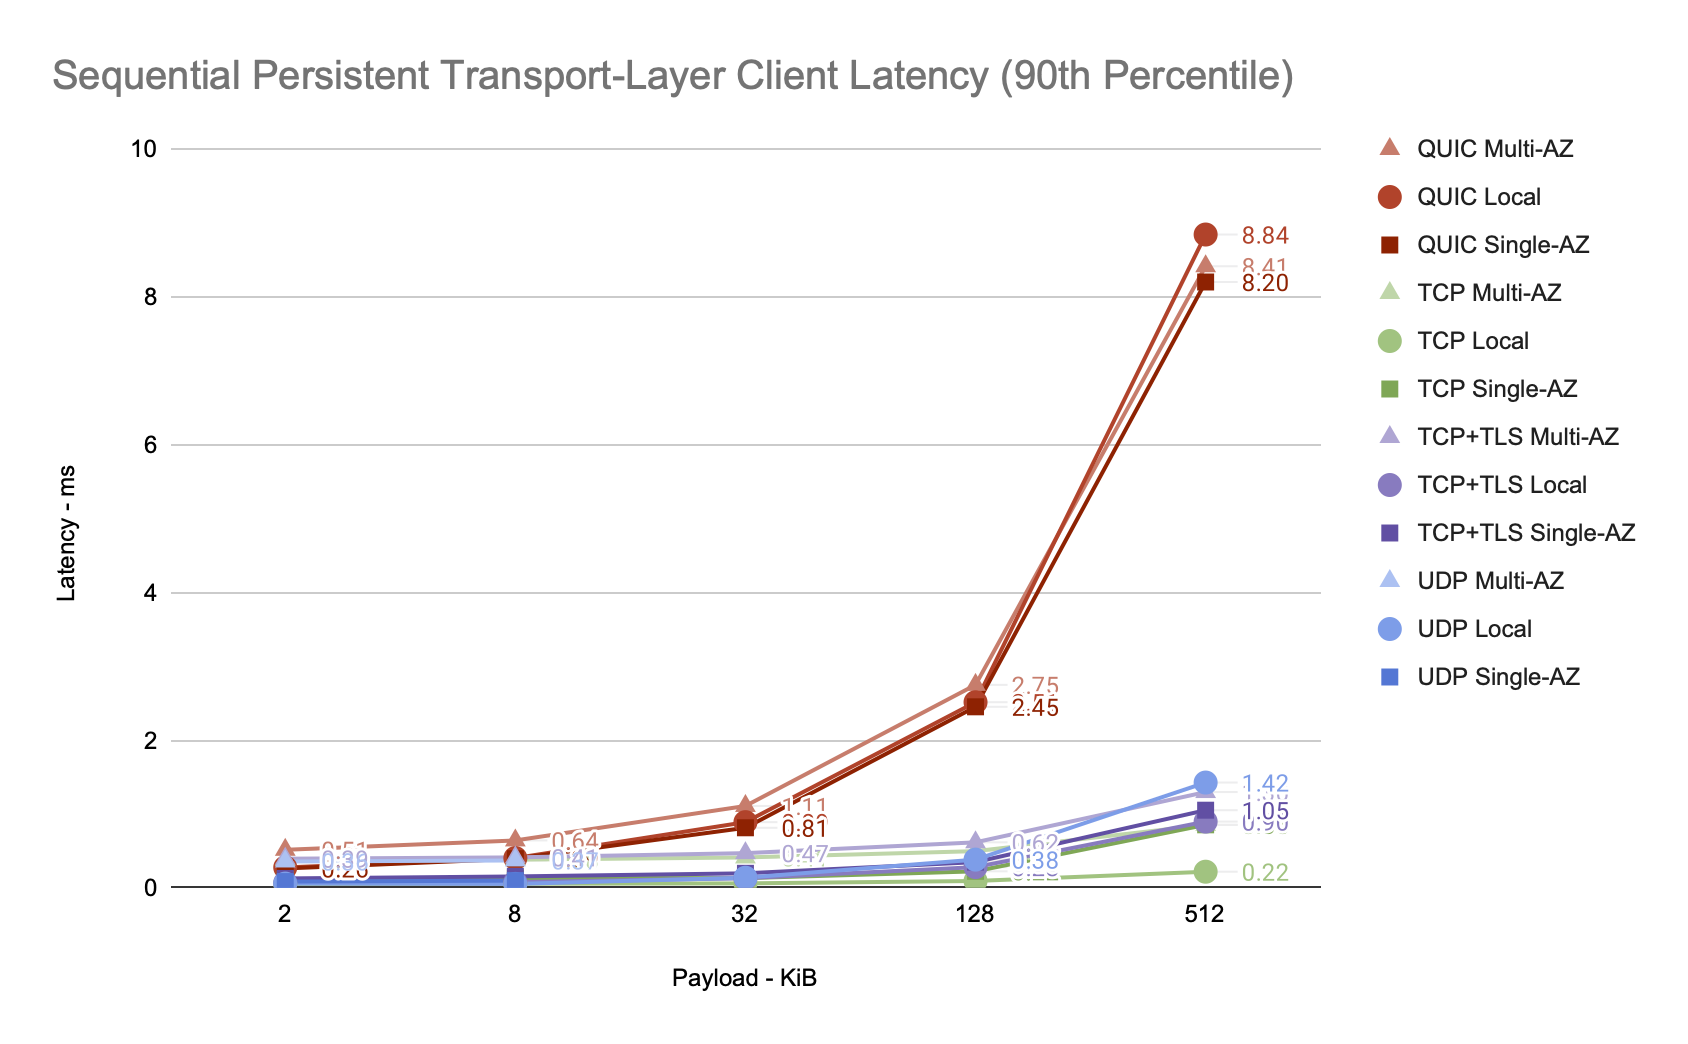
\includegraphics[width=\linewidth]{figures/charts/Sequential Persistent Transport-Layer Client Latency (90th Percentile).png}
    \caption{Sequential Transport-Layer Client Latency (90th Percentile)}
    \label{fig:sequential_transport_latency}
\end{figure}
\begin{figure}
    \centering
    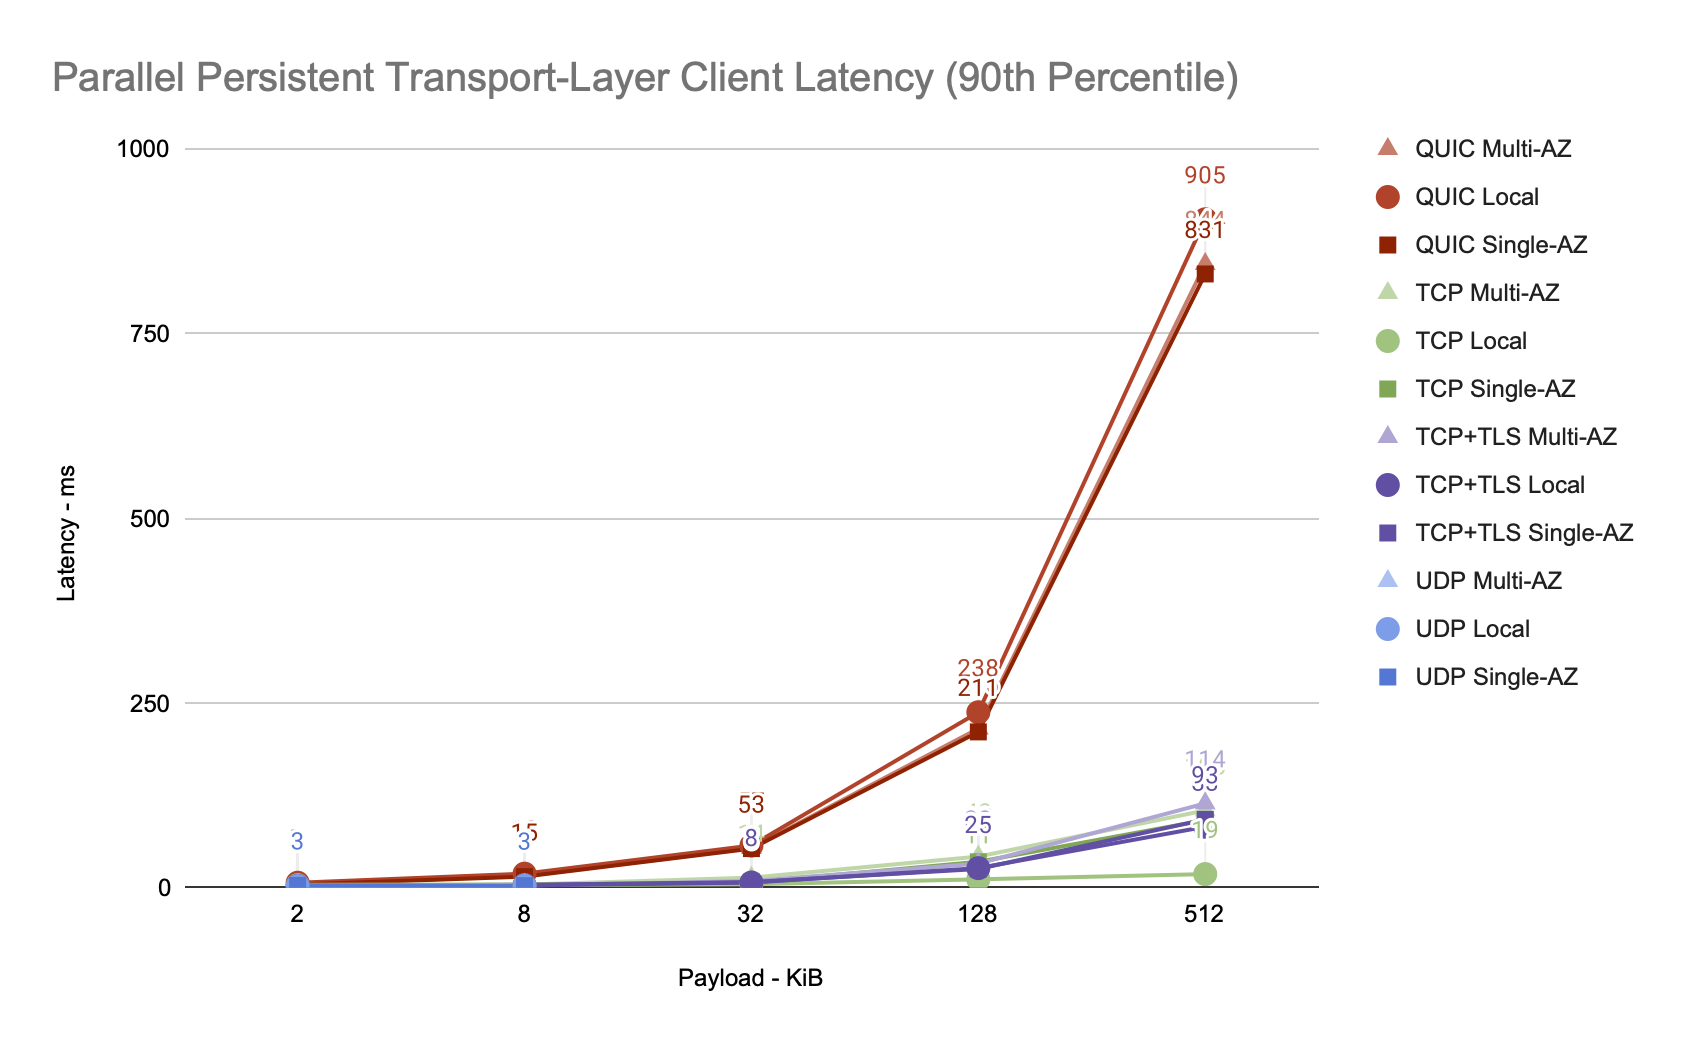
\includegraphics[width=\linewidth]{figures/charts/Parallel Persistent Transport-Layer Client Latency (90th Percentile).png}
    \caption{Parallel Transport-Layer Client Latency (90th Percentile)}
    \label{fig:parallel_transport_latency}
\end{figure}

\begin{figure}[h!]
    \centering
    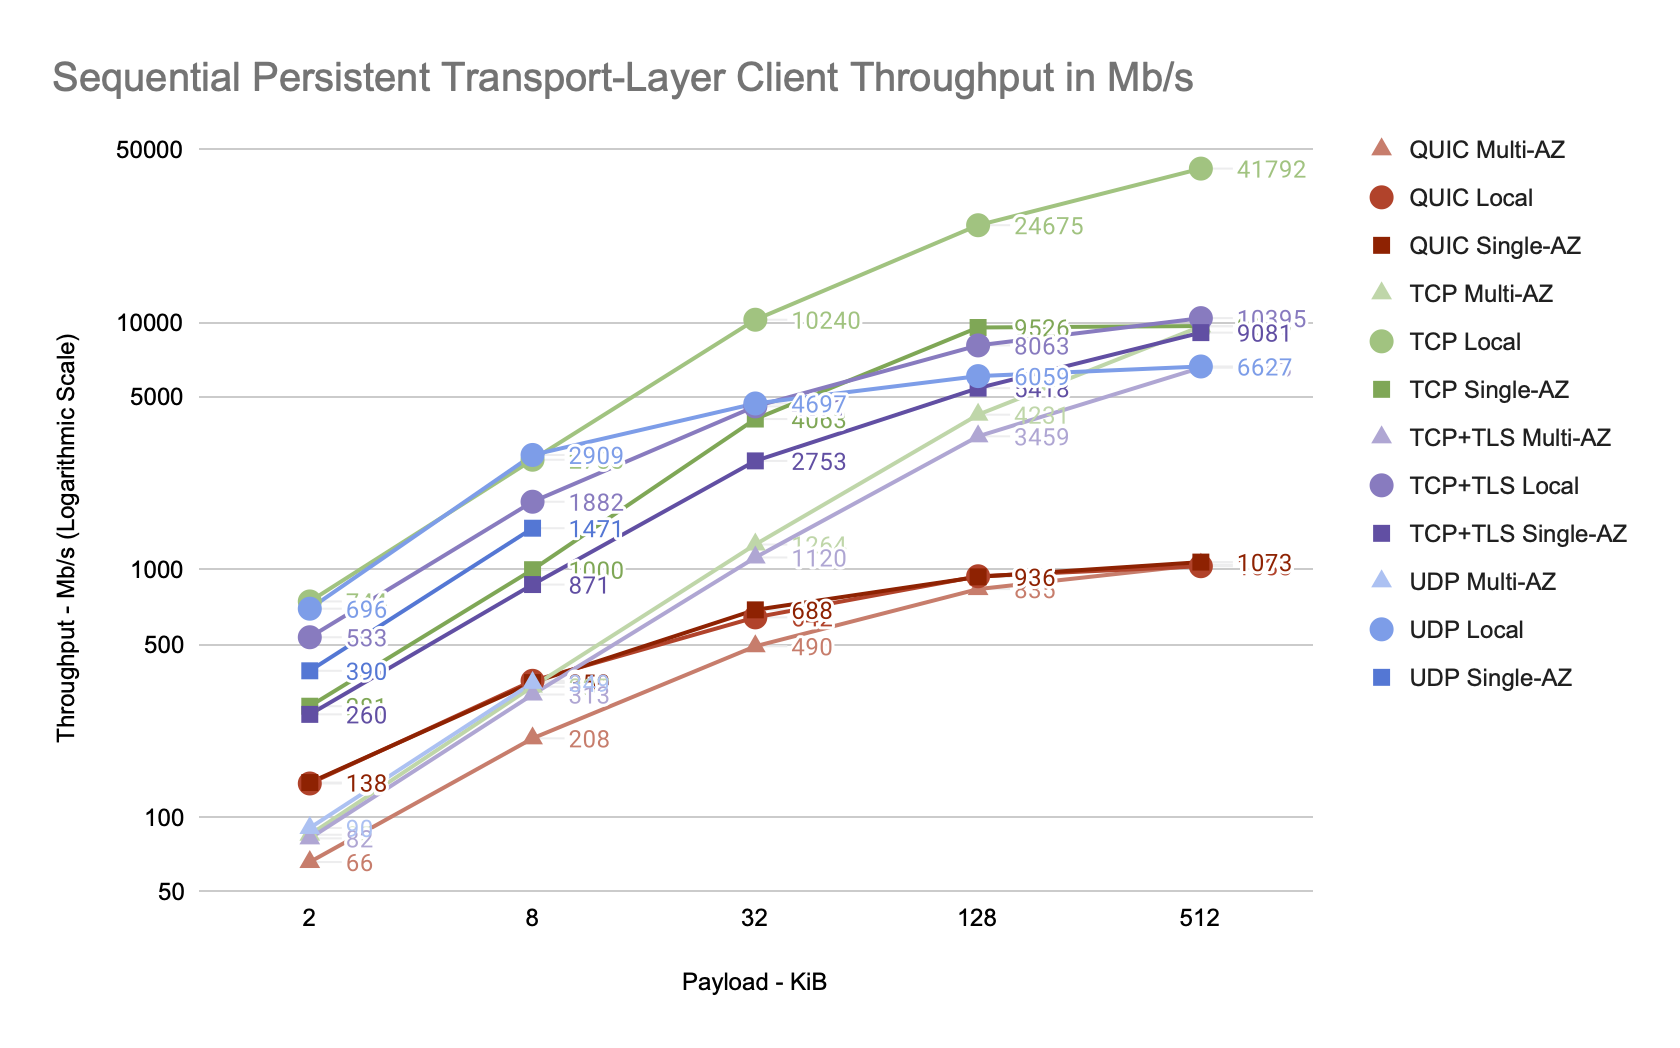
\includegraphics[width=\linewidth]{figures/charts/Sequential Persistent Transport-Layer Client Throughput in Mb_s.png}
    \caption{Sequential Persistent Transport-Layer Client Throughput in Mb/s}
    \label{fig:sequential_transport_throughput}
\end{figure}
\begin{figure}[h!]
    \centering
    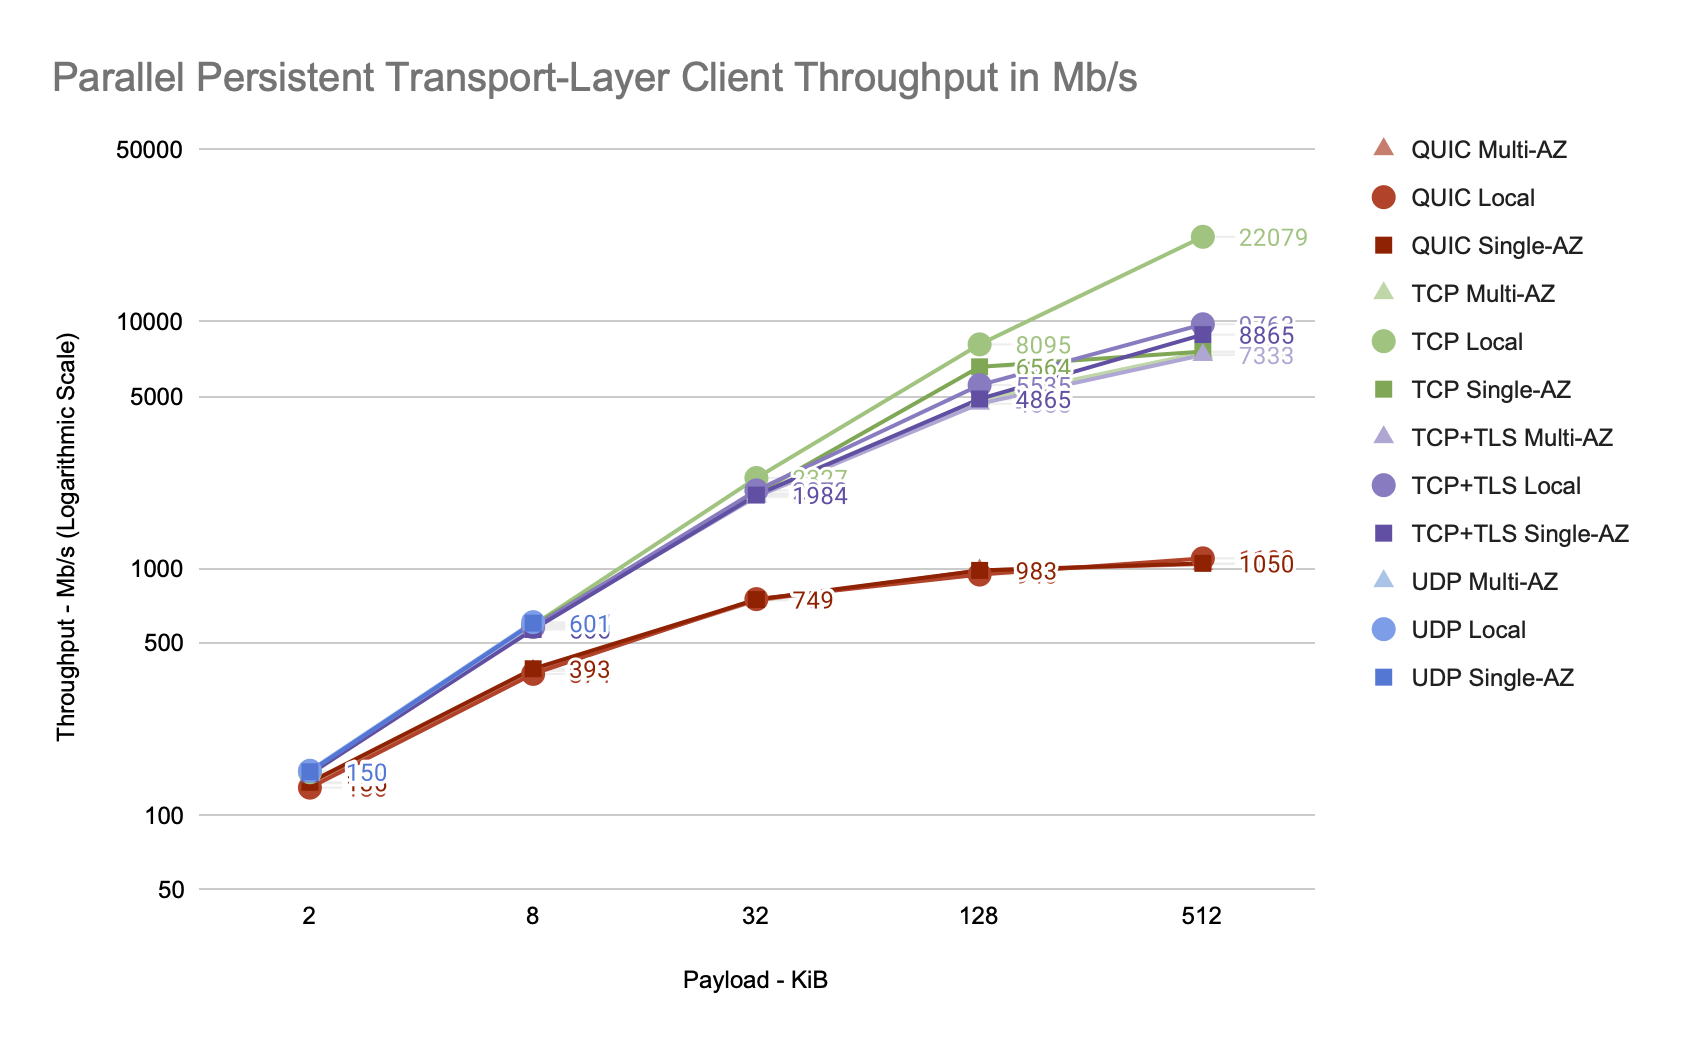
\includegraphics[width=\linewidth]{figures/charts/Parallel Persistent Transport-Layer Client Throughput in Mb_s.png}
    \caption{Parallel Persistent Transport-Layer Client Throughput in Mb/s}
    \label{fig:parallel_transport_throughput}
\end{figure}
